\section{Experimental Profiles}

\subsection{Realistic profile}

The realistic profile samples moderate reviewer skill, substantial noise, nonzero prestige bias, novelty and conformity penalties, publication delay, reviewer labor, reduced attention following rejection, and incomplete resubmission. These ranges are intended as plausible structural values, not fitted estimates.

\subsection{Peer-review-favorable profile}

The stress test deliberately favors peer review:

\begin{itemize}
    \item reviewer skill is near the model maximum;
    \item reviewer noise is near the minimum;
    \item prestige bias, novelty penalties, and conformity incentives are zero;
    \item rejected work retains 75--100\% of normal attention;
    \item revision and resubmission are highly effective;
    \item publication delay and reviewer labor have zero cost;
    \item false recognition receives a high penalty.
\end{itemize}

This profile asks whether an almost ideal gatekeeping system can dominate open alternatives.

\subsection{High-consequence and equity-sensitive profile}

Papers are assigned to basic science, cancer, public health, safety, climate, or infrastructure. Valid high-consequence papers receive larger social-value weights, while false high-consequence papers receive larger harm weights. A disadvantaged-author indicator lowers prestige and presentation resources but does not alter latent truth. The equity gap is

\begin{equation}
\mathcal{E}
=
\Pr(\mathrm{recognized}\mid\mathrm{valid,advantaged})
-
\Pr(\mathrm{recognized}\mid\mathrm{valid,disadvantaged}).
\end{equation}

The consequence-sensitive score penalizes missed true social value and unequal recognition:

\begin{equation}
S_H
=1.4\mathcal{R}_H
-\mathcal{F}_H
-1.3(1-\mathcal{R}_H)
-0.8\mathcal{E}
-0.5\mathcal{C}
-w_DD.
\end{equation}

\subsection{Empirical reviewer-behavior calibration}

A separate calibration layer constrains the reviewer submodel to controlled-study observables rather than assigning empirical percentages directly to latent coefficients. The target file records the epistemic status, tolerance, and source for each observable. Primary targets are the mean major-error detection rate of $2.58/9$ reported by Schroter et al.~\cite{schroter2008}, mean inter-reviewer reliability of $0.34$ and Cohen's kappa of $0.17$ from the meta-analysis by Bornmann et al.~\cite{bornmann2010}, and the positive-versus-null publication recommendation rates of $0.973$ and $0.800$ reported by Emerson et al.~\cite{emerson2010}. Detection among reviewers recommending rejection, $0.391$, is used as a secondary target from Baxt et al.~\cite{baxt1998}. The null baseline for blinding and signing effects follows the planted-error randomized trial of Godlee et al.~\cite{godlee1998}; it is treated as an empirically bounded baseline rather than proof of an exact zero effect.

The internal parameter vector $\theta$ is fitted by rejection approximate Bayesian computation with common random numbers. Candidate parameter sets are scored by

\begin{equation}
L(\theta)=\sum_j
\left(
\frac{\widehat y_j(\theta)-y_j}{\delta_j}
\right)^2,
\end{equation}

where $y_j$ is an empirical observable, $\delta_j$ is its declared calibration tolerance, and $\widehat y_j(\theta)$ is the corresponding simulated observable. The retained sets are parameter combinations consistent with the selected targets; they are not direct empirical estimates of latent coefficients and are not a full Bayesian posterior.

\begin{table}[ht]
\centering
\caption{Controlled-study targets and best-fitting reviewer-submodel observables.}
\label{tab:empiricalcalibration}
\small
\begin{tabular}{lrr}
\toprule
Observable & Empirical target & Best-fitting simulation\\
\midrule
Major-error detection & 0.2867 & 0.2955\\
Inter-reviewer reliability & 0.3400 & 0.3079\\
Cohen's kappa & 0.1700 & 0.1904\\
Positive-result recommendation & 0.9730 & 0.9730\\
Null-result recommendation & 0.8000 & 0.8134\\
Detection among rejectors & 0.3910 & 0.3732\\
\bottomrule
\end{tabular}
\end{table}

The best-fitting parameter set is within the declared tolerance for every primary and secondary target. The calibration used 4,000 global candidates followed by four local refinement rounds of 1,500 candidates each, for 10,000 total parameter evaluations and 5,000 simulated calibration manuscripts per evaluation design.

\begin{figure}[ht]
\centering
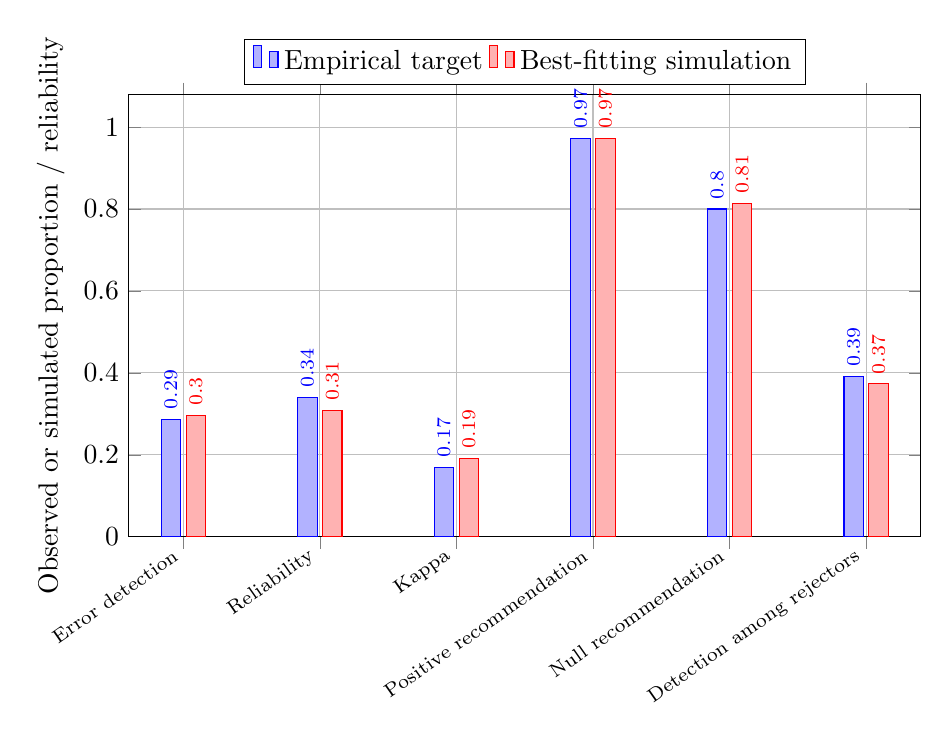
\begin{tikzpicture}
\begin{axis}[
    ybar,
    width=0.96\linewidth,
    height=7.2cm,
    ymin=0, ymax=1.08,
    ylabel={Observed or simulated proportion / reliability},
    symbolic x coords={Error detection,Reliability,Kappa,Positive recommendation,Null recommendation,Detection among rejectors},
    xtick=data,
    x tick label style={rotate=35,anchor=east,font=\scriptsize},
    legend style={at={(0.5,1.02)},anchor=south,legend columns=2},
    nodes near coords,
    nodes near coords style={font=\scriptsize,rotate=90,anchor=west},
    bar width=7pt,
    enlarge x limits=0.08,
    grid=major
]
\addplot coordinates {(Error detection,0.2867) (Reliability,0.3400) (Kappa,0.1700) (Positive recommendation,0.9730) (Null recommendation,0.8000) (Detection among rejectors,0.3910)};
\addplot coordinates {(Error detection,0.2955) (Reliability,0.3079) (Kappa,0.1904) (Positive recommendation,0.9730) (Null recommendation,0.8134) (Detection among rejectors,0.3732)};
\legend{Empirical target,Best-fitting simulation}
\end{axis}
\end{tikzpicture}
\caption{Empirical targets compared with the best-fitting simulated reviewer observables. The calibration matches observable behavior; it does not identify the complete scientific ecosystem.}
\label{fig:empiricalcalibration}
\end{figure}

The calibration is intentionally modular. Reviewer detection, disagreement, and outcome bias are empirically constrained, while post-rejection attention loss, abandonment, long-run discoverability, latent truth prevalence, open-triage effectiveness, and social-value weights remain partially identified, illustrative, or normative. The headline institutional results below therefore remain structural counterfactuals until those ecosystem quantities are calibrated.

\section{Results}

\subsection{Realistic versus idealized conditions}

Table~\ref{tab:profiles} reports simulations of 500 worlds per profile, 250 papers per world, and 25 periods. The realistic and idealized profiles therefore contain 125,000 unique papers each.

\begin{table}[ht]
\centering
\caption{Institutional performance under realistic and peer-review-favorable profiles.}
\label{tab:profiles}
\small
\begin{tabular}{llrrrr}
\toprule
Profile & System & Win share & True value & False recognition & Calibration MSE\\
\midrule
Realistic & Open triage & 52.2\% & 85.0\% & 0.013\% & 0.0331\\
Realistic & Hybrid & 29.4\% & 84.3\% & 0.037\% & 0.0330\\
Realistic & Open & 17.2\% & 81.8\% & 0.082\% & 0.0375\\
Realistic & Peer review & 1.2\% & 72.1\% & 0.460\% & 0.0644\\
\midrule
Idealized & Open triage & 41.2\% & 88.8\% & 0.0075\% & 0.0225\\
Idealized & Peer review & 32.8\% & 88.6\% & 0.018\% & 0.0224\\
Idealized & Hybrid & 22.8\% & 88.1\% & 0.066\% & 0.0241\\
Idealized & Open & 3.2\% & 77.1\% & 0.225\% & 0.0467\\
\bottomrule
\end{tabular}
\end{table}

Under realistic assumptions, traditional peer review recovered substantially less true value, exhibited worse calibration, and won only 1.2\% of worlds. Under the deliberately favorable profile, peer review became competitive with open triage. It did not clearly dominate, despite receiving unusually favorable assumptions and zero cost for delay and labor.

The interpretation is not that expert criticism is harmful. Expert criticism is retained throughout the comparison. The game-theoretic claim concerns the additional veto: when the same evaluative capability can operate without blocking dissemination, attaching gatekeeping power to an imperfect preliminary judgment changes incentives and attention toward a worse system-level outcome. When rejected work retains nearly equal attention and reviewers are unusually accurate and unbiased, the gate's damage becomes smaller. When rejection reduces later evaluation, false negatives persist because evidence cannot accumulate.


\begin{figure}[ht]
\centering
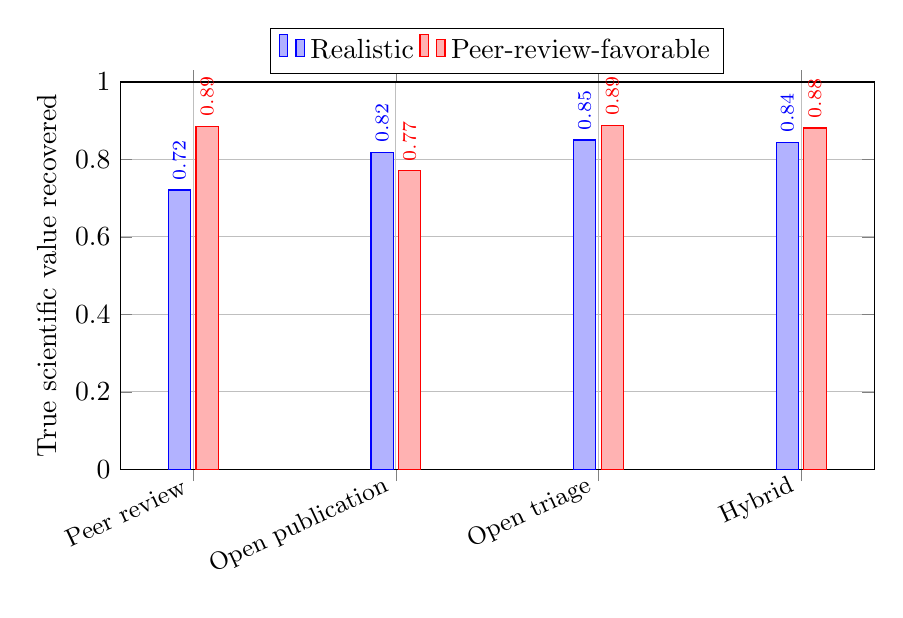
\begin{tikzpicture}
\begin{axis}[
    ybar, width=0.92\linewidth, height=6.5cm, ymin=0, ymax=1.0,
    ylabel={True scientific value recovered},
    symbolic x coords={Peer review,Open publication,Open triage,Hybrid}, xtick=data,
    x tick label style={rotate=25,anchor=east,font=\small},
    legend style={at={(0.5,1.02)},anchor=south,legend columns=2},
    nodes near coords, nodes near coords style={font=\scriptsize,rotate=90,anchor=west},
    bar width=8pt, enlarge x limits=0.12, grid=major
]
\addplot coordinates {(Peer review,0.7213) (Open publication,0.8179) (Open triage,0.8504) (Hybrid,0.8433)};
\addplot coordinates {(Peer review,0.8860) (Open publication,0.7706) (Open triage,0.8876) (Hybrid,0.8814)};
\legend{Realistic,Peer-review-favorable}
\end{axis}
\end{tikzpicture}
\caption{True-value recovery under the realistic and idealized profiles. The large realistic gap between peer review and open triage narrows only under unusually favorable assumptions for gatekeeping.}
\label{fig:profiles_truevalue}
\end{figure}

\subsection{Peer-review-favorable stress test}

A separate 1,000-world stress test used 300 papers and 30 periods per world, yielding 300,000 unique papers. Peer review won 34.4\% of worlds, open triage won 36.6\%, hybrid won 25.6\%, and unfiltered open publication won 3.4\%. Average scores for peer review and open triage were 0.8303 and 0.8318, respectively. Peer review therefore approached parity only after bias, novelty penalties, labor costs, delay costs, and most post-rejection attention losses were removed.


\subsection{Symmetric correction stress test}

The symmetric extension was run for 500 worlds, 250 papers per world, and 25 periods, totaling 125,000 unique papers. All systems could detect and repair methodological, statistical, reporting, and reproducibility defects, and all could introduce harmful revisions.

\begin{table}[ht]
\centering
\caption{Symmetric correction experiment.}
\label{tab:symmetric}
\small
\begin{tabular}{lrrrr}
\toprule
System & Win share & True value & False recognition & Calibration MSE\\
\midrule
Open triage & 55.0\% & 87.2\% & 0.030\% & 0.0311\\
Hybrid & 26.8\% & 86.2\% & 0.110\% & 0.0319\\
Open review & 17.8\% & 84.4\% & 0.080\% & 0.0340\\
Peer review & 0.4\% & 75.1\% & 0.710\% & 0.0696\\
\bottomrule
\end{tabular}
\end{table}

Giving peer review a genuine manuscript-correction mechanism did not reverse the result. The same expert actions were also available after immediate publication, while the peer-review gate continued to reduce subsequent attention to rejected papers. Traditional peer review ended with a mean rejection share of 44.8\%.


\begin{figure}[ht]
\centering
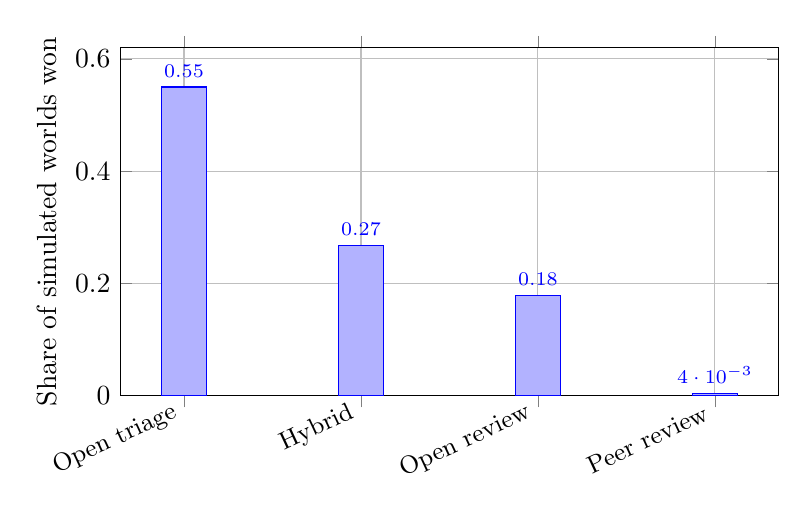
\begin{tikzpicture}
\begin{axis}[
    ybar, width=0.82\linewidth, height=6.0cm, ymin=0, ymax=0.62,
    ylabel={Share of simulated worlds won},
    symbolic x coords={Open triage,Hybrid,Open review,Peer review}, xtick=data,
    x tick label style={rotate=25,anchor=east,font=\small},
    nodes near coords, nodes near coords style={font=\scriptsize},
    bar width=16pt, enlarge x limits=0.12, grid=major
]
\addplot coordinates {(Open triage,0.550) (Hybrid,0.268) (Open review,0.178) (Peer review,0.004)};
\end{axis}
\end{tikzpicture}
\caption{Win shares in the symmetric correction experiment. Once all systems can repair manuscripts, open triage still dominates because expert correction is preserved without allowing an early gate to redirect later attention.}
\label{fig:symmetric_wins}
\end{figure}

\subsection{Equal-total-labor peer-review-favorable test}

The strongest adversarial test used 800 worlds, 220 papers per world, and 24 periods, totaling 176,000 unique papers. Reviewers were strong but not perfect, repair was effective, institutional biases were small, resubmission was easy, rejected papers retained substantial attention, false recognition was penalized heavily, and delay received almost no penalty. Initial review, resubmission review, and continuing evaluation were charged against the same lifetime expert-action budget for every system.

\begin{table}[ht]
\centering
\caption{Peer-review-favorable experiment under exact equal lifetime expert labor.}
\label{tab:equalbudget}
\small
\begin{tabular}{lrrrrr}
\toprule
System & Win share & True value & False recognition & Calibration MSE & Actions\\
\midrule
Open triage & 60.1\% & 90.4\% & 0.001\% & 0.0244 & 5018.0\\
Hybrid & 18.1\% & 88.5\% & 0.070\% & 0.0273 & 5018.0\\
Peer review & 14.0\% & 88.5\% & 0.160\% & 0.0324 & 5018.0\\
Open review & 7.8\% & 85.8\% & 0.049\% & 0.0315 & 5018.0\\
\bottomrule
\end{tabular}
\end{table}

Peer review remained useful and recovered nearly as much true value as the hybrid system, but it did not become the optimal institution. Its mean final rejection share was 46.7\%. The experiment isolates the distinction between expert criticism and gatekeeping: correction remained valuable, while making a noisy preliminary decision control later attention remained costly.


\begin{figure}[ht]
\centering
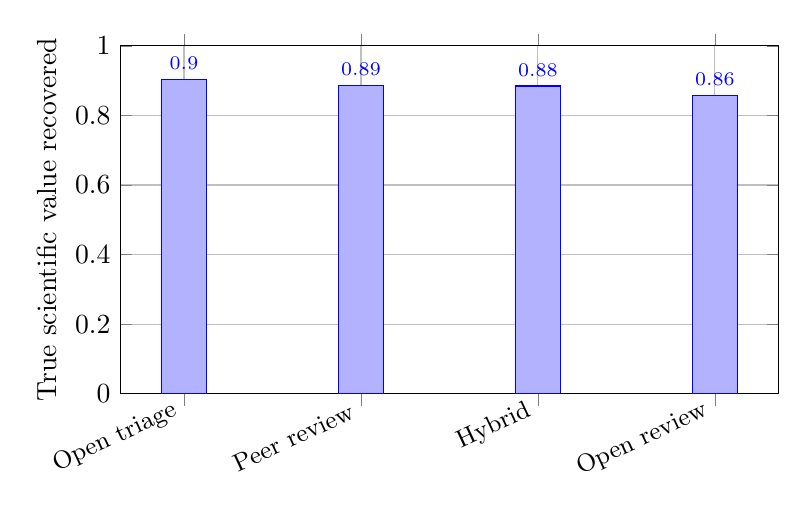
\begin{tikzpicture}
\begin{axis}[
    ybar, width=0.82\linewidth, height=6.0cm, ymin=0, ymax=1.0,
    ylabel={True scientific value recovered},
    symbolic x coords={Open triage,Peer review,Hybrid,Open review}, xtick=data,
    x tick label style={rotate=25,anchor=east,font=\small},
    nodes near coords, nodes near coords style={font=\scriptsize},
    bar width=16pt, enlarge x limits=0.12, grid=major
]
\addplot coordinates {(Open triage,0.9037) (Peer review,0.8854) (Hybrid,0.8846) (Open review,0.8582)};
\end{axis}
\end{tikzpicture}
\caption{True-value recovery in the exact equal-lifetime-labor stress test. Even after constraining all systems to the same lifetime expert-action budget, open triage recovers the most hidden true value.}
\label{fig:equalbudget_truevalue}
\end{figure}

\subsection{High-consequence and equity-sensitive simulation}

Table~\ref{tab:harm} reports 1,000 worlds, 300 papers per world, and 30 periods, totaling 300,000 unique papers.

\begin{table}[ht]
\centering
\caption{High-consequence and equity-sensitive results.}
\label{tab:harm}
\small
\begin{tabular}{lrrrrr}
\toprule
System & Win share & True social value & Missed true harm & False harm & Equity gap\\
\midrule
Open triage & 40.5\% & 84.7\% & 15.3\% & 0.0017\% & 2.50\%\\
Hybrid & 38.8\% & 84.5\% & 15.5\% & 0.018\% & 2.45\%\\
Open & 19.0\% & 82.3\% & 17.8\% & 0.084\% & 4.17\%\\
Peer review & 1.7\% & 72.8\% & 27.2\% & 0.424\% & 8.79\%\\
\bottomrule
\end{tabular}
\end{table}

When false-negative costs were allowed to reflect high-stakes domains, peer review lost 27.2\% of available true social value. Its equity gap was more than three times that of the hybrid and open-triage systems. The model also produced a higher realized false-harm rate under peer review because preliminary certification concentrated attention and confidence around some accepted false claims, while valid rejected claims received less opportunity to accumulate evidence.


\begin{figure}[ht]
\centering
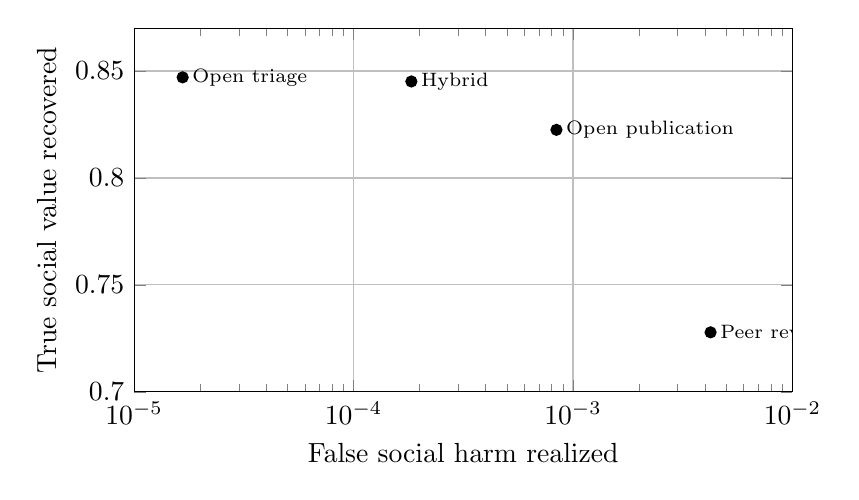
\begin{tikzpicture}
\begin{axis}[
    width=0.82\linewidth, height=6.2cm, xmode=log,
    xlabel={False social harm realized}, ylabel={True social value recovered},
    xmin=0.00001, xmax=0.01, ymin=0.70, ymax=0.87, grid=major
]
\addplot[only marks,mark=*] coordinates {(0.0000166485,0.847041) (0.000183478,0.845108) (0.000840732,0.822500) (0.00423677,0.727835)};
\node[anchor=west,font=\scriptsize] at (axis cs:0.0000166485,0.847041) {Open triage};
\node[anchor=west,font=\scriptsize] at (axis cs:0.000183478,0.845108) {Hybrid};
\node[anchor=west,font=\scriptsize] at (axis cs:0.000840732,0.822500) {Open publication};
\node[anchor=west,font=\scriptsize] at (axis cs:0.00423677,0.727835) {Peer review};
\end{axis}
\end{tikzpicture}
\caption{High-consequence tradeoff between recovered true social value and realized false social harm. Open triage and the hybrid system occupy the favorable upper-left region.}
\label{fig:highconsequence_tradeoff}
\end{figure}
